\begin{center}
  \Large
  \textbf{BIOGRAFI PENULIS}
\end{center}

\addcontentsline{toc}{chapter}{BIOGRAFI PENULIS}

\vspace{2ex}

\begin{wrapfigure}{L}{0.3\textwidth}
  \centering
  \vspace{-3ex}
  % Ubah file gambar berikut dengan file foto dari mahasiswa
  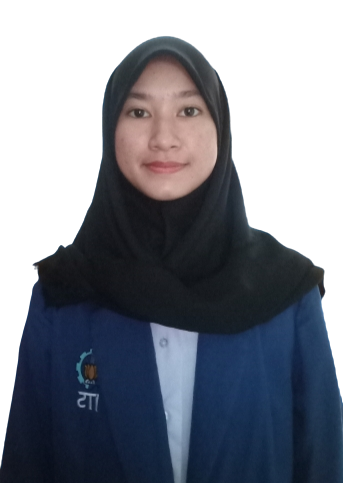
\includegraphics[width=0.3\textwidth]{gambar/formal.png}
  \vspace{-4ex}
\end{wrapfigure}

% Ubah kalimat berikut dengan biografi dari mahasiswa
\name{}, lahir di Gresik pada 2 November 2000. Penulis telah menempuh beberapa jenjang Pendidikan formal di 
beberapa sekolah yaitu: SMPN 2 Sidoarjo (2013-2016), dan SMAN 2 Sidoarjo (2016-2019). Penulis melanjutkan 
Pendidikan sarjana di Departemen Teknik Komputer Fakultas Teknologi Elektro dan Informatika Cerdas (FTEIC) 
Institut Teknologi Sepuluh Nopember (ITS) pada tahun 2019 yang terdaftar sebagai mahasiswa dengan nomor 
mahasiswa 07211940000017. Selama menjadi mahasiswa, penulis aktif mengikuti kegiatan kepanitiaan diantaranya Evolve,
MAGE 6, dan MAGE 7. Penulis juga aktif mengikuti beberapa organisasi seperti menjadi Bendahara di 
Himpunan Mahasiswa Teknik Komputer (HIMATEKKOM). Penulis tertarik dengan bidang machine learning dan pengembangan web.
Untuk mendapatkan gelar S.T (Sarjana Teknik), penulis mengambil topik penelitian tugas akhir deep learning khususnya 
yang berkaitan dengan IndRNN. Untuk kepentingan penelitian, pembaca yang memiliki kritik, saran, atau pertanyaan 
mengenai tugas akhir ini dapat menghubungi penulis melalui email adritiamerdila.19072@mhs.its.ac.id.

